%!TEX program = xelatex
\documentclass[twoside,color=blue,mathpazo,titlestyle=hang,12pt]{elegantbook}
% \email{elegantlatex2e@gmail.com}
% \title{统计观点下的测量平差}
% \zhtitle{统计观点下的测量平差}
% \zhend{}
% \entitle{\ }
% \enend{}
% \version{2.10}
% \myquote{Victory won\rq t come to us unless we go to it.}
% \logo{logo.pdf}
% \cover{cover.pdf}

% title 
\setcounter{tocdepth}{2}
\numberwithin{equation}{section}


\title{{\Huge\emph{2018年GIS课程设计}\\实验报告}\\{\Large 项目名称:测量全生命周期支持系统}}
\author
{
\Large\textbf{同济大学测绘与地理信息学院} \\
1551126 余周炜 \\
王雪辰 \\
江子宇
}
\date{}

%green color
%    \definecolor{main1}{RGB}{0,120,2}
%    \definecolor{seco1}{RGB}{230,90,7}
%    \definecolor{thid1}{RGB}{0,160,152}

   \definecolor{main1}{RGB}{0,0,0}
   \definecolor{seco1}{RGB}{0,0,0}
   \definecolor{thid1}{RGB}{0,0,0}
%cyan color
   \definecolor{main2}{RGB}{0,175,152}
   \definecolor{seco2}{RGB}{239,126,30}
   \definecolor{thid2}{RGB}{120,8,13}
%blue color
   \definecolor{main3}{RGB}{100,149,237}
   \definecolor{seco3}{RGB}{180,50,131}
   \definecolor{thid3}{RGB}{7,127,128}

\usepackage{siunitx}
\usepackage[section]{placeins}
\usepackage{makecell}
\usepackage{listings}

\newcommand\mgape[1]{\gape{$\vcenter{\hbox{#1}}$}}

\newfontfamily\conso{Inconsolata}
\definecolor{mygreen}{rgb}{0,0.6,0}
\definecolor{mygray}{rgb}{0.5,0.5,0.5}
\definecolor{mymauve}{rgb}{0.58,0,0.82}
\lstset{backgroundcolor=\color{white},
numbers=left,
numberstyle=\small,
frame=lines,
basicstyle=\conso,
columns=fullflexible,
breaklines=true,                 % automatic line breaking only at whitespace
tabsize=4,
keywordstyle=\color{blue},
commentstyle=\color{mygreen},
stringstyle=\color{mymauve}\ttfamily,
language=Matlab}
% \usepackage[numbered,autolinebreaks,useliterate]{mcode}

% \usepackage{mdwlist}
\usepackage{lipsum}
\usepackage{colortbl}
\usepackage{texnames}
\usepackage{metalogo}
\usepackage{mflogo}
\usepackage{mathtools}
\usepackage{algorithm}
% \usepackage{algorithmicx}
\usepackage{algpseudocode}
\usepackage{longtable}
\usepackage{supertabular}
\usepackage{multirow}
\renewcommand{\algorithmicrequire}{\textbf{Input:}}  % Use Input in the format of Algorithm  
\renewcommand{\algorithmicensure}{\textbf{Output:}} % Use Output in the format of Algorithm 


\RequirePackage{cite}
\RequirePackage[square,numbers]{natbib}
\newlength{\notationgap}
\setlength{\notationgap}{1pc}

\newlength{\figwidth}
\setlength{\figwidth}{26pc}

\begin{document}
\frontmatter

\maketitle

\include{math_symbol}
\tableofcontents

\mainmatter

\chapter{项目简介}

本项目的名称是“测量全生命周期支持系统”,使用vs2010+arcEngine10.1开发,分为两个部分,一部分进行\textbf{辅助测量},是为测量辅助系统,另一部分\textbf{生成等高线}。

本项目的背景如下:测量实习中,我们常常为找不到控制点和输入新的控制点而烦恼,也为后面建立等高线的繁琐操作而苦恼不已,为了解决测量实习中的问题,开发了本系统,将测量过程中的各种操作用ArcEngine开发解决,使测量过程更加简单流畅。具体实现的功能将在后面的部分介绍。


本项目主要有三个窗体,Form1为主窗体,如图\ref{fig:mainform}所示。
\begin{figure}[htbp]
\caption{主窗体}
\label{fig:mainform}
\centering
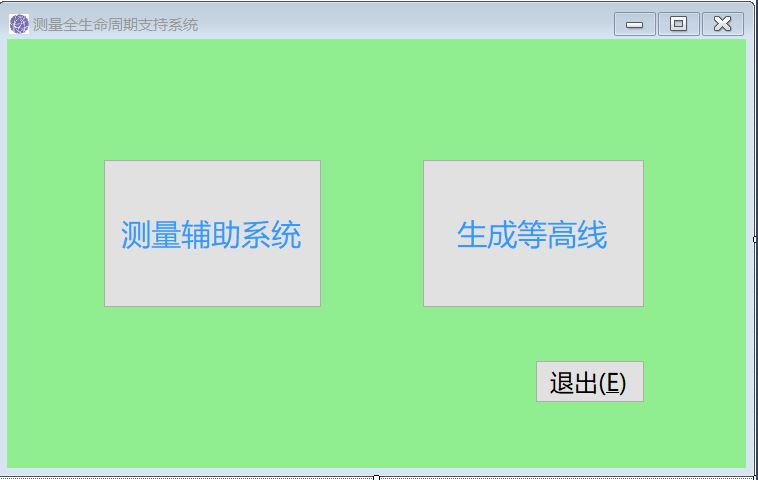
\includegraphics[width=0.8\textwidth]{mainform.JPG}
\end{figure}

第二个窗体是FormSurvey,辅助有关测量行为的进行,如图\ref{fig:forms}所示。
\begin{figure}[htbp]
\caption{FormSurvey}
\label{fig:forms}
\centering
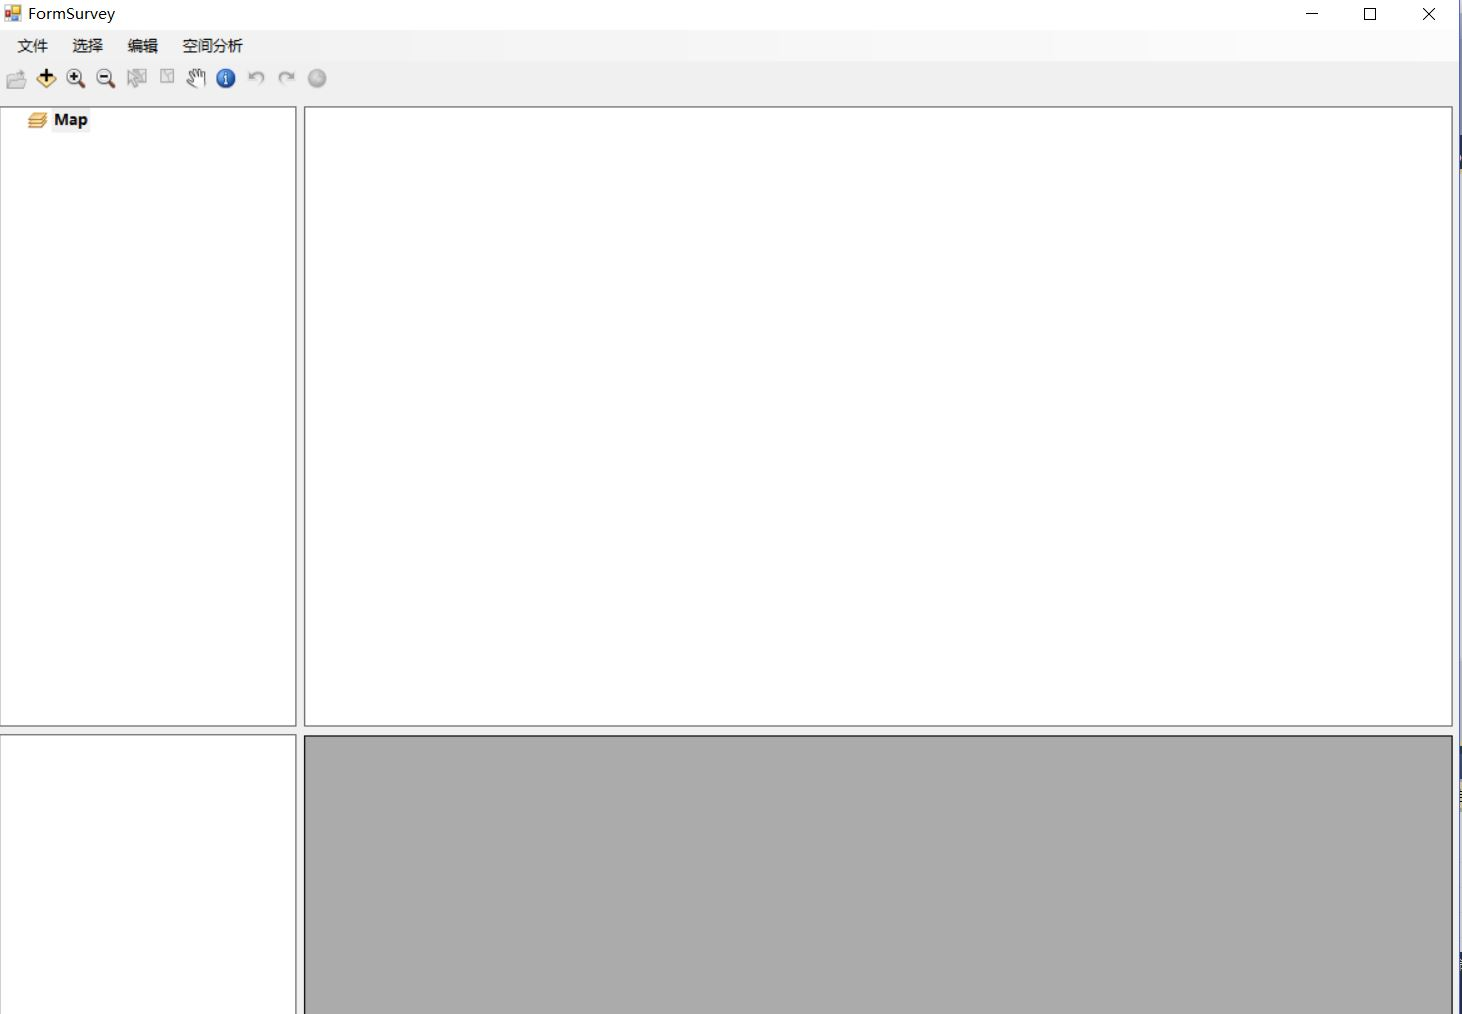
\includegraphics[width=0.8\textwidth]{forms.JPG}
\end{figure}

第三个窗体是FormCoutour,进行有关等高线的绘制,如图\ref{fig:formc}所示。
\begin{figure}[htbp]
\caption{FormCoutour}
\label{fig:formc}
\centering
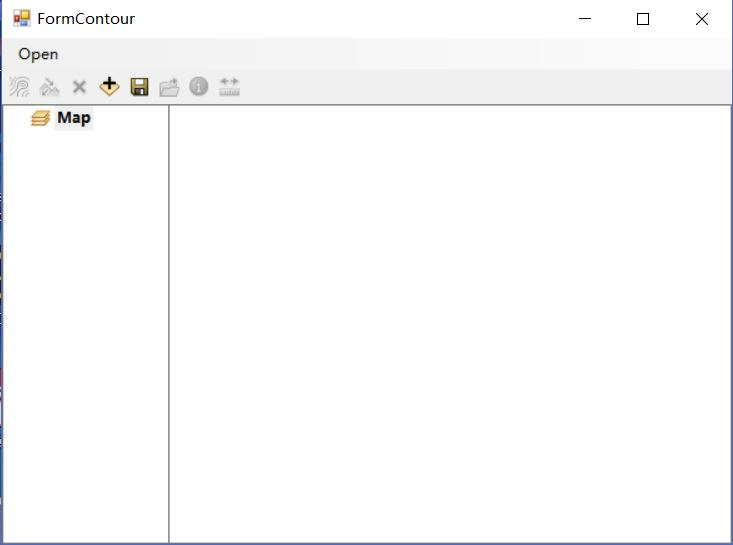
\includegraphics[width=0.8\textwidth]{formc.JPG}
\end{figure}

此外还有FormDistance,AddControlPoint等对话框。

\chapter{测量辅助系统}

测量辅助系统实现了如下特色功能
\begin{enumerate}   
\item 鹰眼功能。
\item 鼠标拖动移动图层功能。
\item 输入坐标的方式添加控制点。
\item 拉框选择测区范围,显示测区边界,并将测区范围内的控制点高亮显示。
\item 选择测站所在的控制点、输入测距,在考虑遮蔽和测距的前提下给出可用的后视点。
\item 选中测站所在的控制点,给出测区范围。
\end{enumerate}

下面分别说明这些功能
\begin{description}
\item[鹰眼功能] 
\end{description}






    

\chapter{构思}

本程序分为三个部分,一是主界面,二是shp部分,第三是等高线部分。

\begin{enumerate}
\item 界面
\item shp部分(数据集 控制点shp+polygon shp)
\begin{enumerate}
\item 鹰眼功能
\item 拉框选择测区范围,在图上显示该测区所有控制点
\item 选中某一控制点 给出可用的后视点 (遮蔽问题 满足一定距离)
\item 选中某一控制点 给出测区范围     (缓冲区 遮蔽问题)
\item 添加控制点 方式 输入坐标
\end{enumerate}
\item 等高线部分
\begin{enumerate}
\item 建TIN
\item TIN转栅格
\item 生成等高线
\end{enumerate}
\end{enumerate}
   

\chapter{小组特色}

本小组通过不断学习尝试,实现了如下特色功能:
\begin{enumerate}
\item 鼠标拖拽使图层上下移动
\end{enumerate}

% \bibliographystyle{plainnat}
% \bibliography{reference}
% \addcontentsline{toc}{chapter}{参考文献}

\end{document}
